\documentclass[12pt,english]{article}
\usepackage{geometry}
\geometry{verbose, letterpaper, tmargin = 2.54cm, bmargin = 2.54cm,
  lmargin = 2.54cm, rmargin = 2.54cm}
\geometry{letterpaper}
\usepackage{graphicx}
\usepackage{amsmath}
\usepackage{setspace}
\usepackage{url}
\usepackage{lineno}
\usepackage{xcolor}
\usepackage{bm}
\renewcommand\linenumberfont{\normalfont\tiny\sffamily\color{gray}}
\modulolinenumbers[2]

% Linux Libertine:
\usepackage{textcomp}
\usepackage[sb]{libertine}
\usepackage[varqu,varl]{inconsolata}% sans serif typewriter
\usepackage[libertine,bigdelims,vvarbb]{newtxmath} % bb from STIX
\usepackage[cal=boondoxo]{mathalfa} % mathcal
\useosf % osf for text, not math
\usepackage[supstfm=libertinesups,%
  supscaled=1.2,%
  raised=-.13em]{superiors}

\textheight 22.0cm

\usepackage[round,sectionbib]{natbib}
\bibpunct{(}{)}{;}{a}{}{;}
\bibliographystyle{mee}

\title{Modelling spatiotemporal extremes in ecology}
\author{
Sean C. Anderson$^1$ and
Eric J. Ward$^2$
}
\date{}

\begin{document}

\maketitle

\begin{spacing}{1.25}

  % Point 1: set the context and purpose for the work; 
% Point 2: indicate the approach and methods used; 
% Point 3: outline the main results; 
% Point 4: identify the conclusions, the wider implications and the relevance to management or policy. 
% •	Key-words: Provide a maximum of 10 keywords or phrases.

\begin{abstract}

Understanding biological responses to environmental perturbations in time and
space is critical for conservation planning. With projected trends in climate
forcing, for example, conservation biology will have to focus not just on mean
changes, but also on variability and extremes. In ecological systems, extremes
can happen in time, such as population crashes, or in space, such as rapid
range contractions. Here, we introduce a statistical model that extends current
methods for joint inference about temporal and spatial dynamics (spatiotemporal
modelling) to allow for and detect extremes that occur simultaneously in time
and space. Specifically, our model is a Bayesian predictive-process model that
uses a multivariate-t distribution to describe spatial random effects. The
model is easily implemented with our flexible new R package \textbf{rrfields},
which uses an interface that should be familiar to anyone who has worked with
regression in R. We illustrate applications of our model and R package simulated and
real-world data. First, we \ldots
Second, we predict tree mortality from mountain pine beetle (\emph{Dendroctonus
  ponderosae}) outbreaks in the US Pacific Northwest over the last 16 years. In
both cases, we show that our model provides more accurate and certain
predictions of these ecological processes compared to traditional
spatiotemporal models that do not allow for extremes. Jointly modelling
ecological processes in time and space represents an important step forward to
creating realistic models of anomalies, and allows us to improve predictions
that feed into conservation decisions. Distributing this tool as an R package
should make these models accessible to a wide range of conservation biologists
and scientists in other disciplines interested in predicting extreme events.
\end{abstract}

\section{Introduction}

Applications of statistical models that allow for joint inference about spatial
and temporal dynamics have advanced rapidly in ecology over the last several
decades \citep{bascompte1995, latimer2009}. Spatiotemporal models have also
been widely used in other disciplines, including applications to weather,
remote sensing, human disease dynamics, and crime \citep{cressie2011}. Many
types of linear and non-linear models that ecologists are accustomed to working
with (e.g.~generalized linear models, generalized additive models) can be
modified to include spatiotemporal components, where spatial processes are
modeled as multivariate random effects. Many of these methods are available in
existing R packages, including but not limited to \textbf{spBayes}
\citep{finley2007}, \textbf{spTimer} \citep{bakar2015}, \textbf{INLA}
\citep{rue2009}, \textbf{RandomFields} \citep{schlather2016}, and
\textbf{spate} \citep{sigrist2015}.

For large datasets that include more than several hundred spatial locations,
estimation of multivariate random effects at the locations of the data may be
computationally prohibitive. One solution to this dimensionality problem is to
estimate the random field as correlated random effects at a smaller subset of
locations or $m$ `knots' \citep[e.g.][]{latimer2009, shelton2014}, where $m
  < n$, the number of data points. The estimated random effects are assumed to
be jointly distributed (e.g.~multivariate normal). Instead of estimating an
unconstrained $m \times m$ covariance matrix, a covariance function is
specified \emph{a priori} to estimate the covariance between locations; this
function may be isotropic (where covariance is a function of distance,
e.g.~exponential or Gaussian) or anisotropic (where covariance also depends on
direction, e.g.~Matern). Given the estimated random effects at the knot
locations, and the known distance matrix between the knots and observed data,
it is straightforward to project or interpolate those random effects to the
locations of observations \citep{latimer2009, finley2009}.

Reducing the spatial dimension of a dataset yields a smaller covariance matrix,
but may still be computationally intensive because the covariance matrix is
dense (most elements are non-zero). For some spatial problems, inference about
the covariance between points separated by large distances may not be of
interest because the correlation is negligible. In geostatistics, the `range'
of a semivariogram is often used to identify thresholds beyond which pairs of
points are not correlated \citep{rossi1992}. A second approach to increase the
efficiency of parameter estimation in spatiotemporal models with large datasets
is to implement models that rely on sparse matrix algorithms. One of the most
recent advances in these class of models is the stochastic partial differential
equation (SPDE) approximation to Gaussian random fields proposed by
\citet{lindgren2011}. These methods have been implemented using the integrated
nested Laplace approximation (INLA) \citep{rue2009}, which allows for
approximate Bayesian inference without Markov chain Monte Carlo (MCMC)
sampling. Use of the SPDE-INLA approach has increased rapidly in ecology over
the last five years \citep[e.g.][]{illian2013, ono2016}.

A limitation of models that include Gaussian random fields is that they may
perform poorly when underlying data include anomalous or extreme events. More
on dragon kings and stuff here? Extreme events in temporal processes have been
modeled using a variety of methods in ecology, typically by including finite
mixtures of normal and
heavy-tailed distributions \citep{everitt1996, ward2007, thorson2011}.
More recently, the use of the Student-t distribution
has been proposed as a robust solution to modeling process variation in
population dynamics (Anderson et al. in press).

Several robust extensions of Gaussian random fields have been proposed to
better model extreme spatial events, including applications of max-stable or
extreme value theory \citep{davison2012, davison2012a}. Many of the
applications of these models, such as understanding extremes in rainfall or
flooding, are interested in quantifying the probabilities of exceeding some
threshold \citep{davis2008}. Other extensions of spatiotemporal models to model
extremes include the use of multivariate-t spatial random fields
\citep{roislien2007}. Focusing on the latter, to our knowledge these methods
have not been considered for data in the ecology, fisheries, or environmental
sciences.

The objectives of this paper are to introduce the use of robust spatial
predictive models using the multivariate-t distribution, easily implemented in
our new R package \textbf{rrfields} (robust random fields). Using simulation
testing to compare the multivariate normal to multivariate-t spatial processes,
we illustrate that the multivariate-t leads to better prediction (less bias,
lower uncertainty). Second, we illustrate applications of these modeling
approaches to real-world data that include spatial extremes, using chlorophyll
data from the west coast of the United States \citep{mckibben2012}, and counts
of European starlings (\emph{Sturnus vulgaris}) from the North American
Breeding Bird Survey \citep{pardieck2016}. These applications differ in their
observation error model (normal, Gamma) and treatment of temporal change,
illustrating the flexibility of these robust spatial models to other
applications in ecology and related fields.

\section{Methods}

\subsection{Overview}

We seek to allow for large deviations in an ecological spatial pattern over
time by extending a spatiotemporal predictive process model to use a MVT
distribution instead of the usual MVN. Below we describe the form of our model
as implemented in \textbf{rrfields}, describe two simulations exploring model
performance, and finally describe the application of our model to a data set
representing mountain pine beetle outbreaks in the Pacific Northwest of the
United States. 

\subsection{The MVT predictive process model}

\citet{latimer2009} provides an excellent description of predictive process
models for ecologists. Below we summarize the important elements of these
models and highlight how our models differs from the usual MVN version. Our
model is essentially a generalized linear model (GLM) with a spatiotemporal
element described by a random field. Our model describes the mean or expected
value of the response, $\mu \equiv \mathbb{E}(y)$, at location in space $s$ and
time $t$ as

\begin{equation}
  g(\mu_{s,t}) = \bm{X}_{s,t} \bm{\beta} + \gamma_{s,t},
\end{equation}

\noindent where $g$ describes a link function (e.g., identity or log),
$\bm{X}_{s,t}$ describes a vector of predictors, and $\bm{\beta}$ describes a
vector of estimated coefficients. The variance of the observation component of
our model, as in any GLM, is described as a function of the mean via a
probability distribution from the exponential family such as the Gaussian,
Poisson, or gamma. The symbol $\gamma$ describes the spatiotemporal process
which we describe below. 

A random field is a term used to describe ``random effects'' drawn from a
multivariate probability distribution. Most commonly, these values are drawn
from a multivariate normal (MVN) with some covariance matrix, $\Sigma$.
Instead, we draw our values from a multivariate t distribution (MVT). The MVT
has one extra parameter compared to the MVN, the degrees of freedom parameter
$\nu$. When $\nu$ is small (say $\nu < 10$) the distribution has heavier
tails than the MVN. As $\nu$ approaches infinity, the distribution approaches
the MVN. For most purposes, the MVT and MVN are indistinguishable for moderate
values of $\nu$ (say $\nu > 20$) similarly to the univariate t-distribution
compared with the univariate normal distribution (REF). 

If $W_{s,t}$ defines a random field, then the spatiotemporal element,
$\gamma_{s,t}$, can be made temporally constant (one field shared across time,
$\gamma_{s,t} = W_{s}$), independent at each time step ($\gamma_{s,t} =
W_{s,t}$) or autoregressive so that the spatial pattern at time $t$ is
dependent on the spatial pattern at time $t-1$ to a degree defined by $\phi$,
($\gamma_{s,t} = \phi \gamma_{s,t-1} + W_{s,t}$). In the last case, in practice,
we constrain the spatiotemporal autoregressive process to be centred on zero at
each time step to aid interpretation and ensure identifiability ($\gamma_{s,t}
= \phi (\gamma_{s,t-1} - \mathbb{E}[\gamma_{t-1}]) + W_{s,t}$). This lets the
mean process be defined by the linear predictor ($\bm{X_{s,t}}\bm{\beta}$)
while $\gamma_{s,t}$ defines the spatial process and how it evolves through
time --- potentially letting ``hotspots'' remain hotspots through time while
keeping the means of the spatial process $\gamma_{s,t}$ stationary and centred
on zero.

We determine the location of the $m$ knots using a partitioning around medoids
algorithm \citep[the \texttt{pam} function in the R package
\textbf{cluster};][]{reynolds2006}. This algorithm is a robust version of the
common k-means algorithm and results in selecting knot locations that are
proportional to spatial sampling intensity. 

We used a squared exponential covariance function to model the correlation
between locations because this is one of the most commonly adopted covariance
functions for spatiotemporal models. The squared exponential function, $H$,
(also known as the Gaussian covariance function) models the correlation between
points $i$ and $j$ as $H(\delta_{ij}) = \exp \left(-\phi \delta_{ij}^2
\right)$, where $\delta_{ij}$ describes the distance between points $i$ and $j$
and $\phi$ describes how steeply correlation declines with increasing distance
or the ``wiggliness'' of the spatial process. Large values of $\phi$ correspond
to XX spatial patterns and small values correspondence to XX spatial patterns.

The elements of the covariance matrix at the $m$ knot locations are therefore
defined as $\Sigma_{ij}^*=\sigma^2 \left( -\phi \delta_{ij}^2 \right)$ with the
parameter $\sigma$ scaling the amplitude of the spatial process deviations. Our
package also allows for the exponential covariance function $H(\delta_{ij}) =
\exp \left(-\phi \delta_{ij} \right)$ and could be extended to allow for other
common covariance functions such as the Matern or anisotropic covariance
functions in which covariance is not uniform in all directions. 
Following \citet{latimer2009}, we can also calculate the covariance matrix
between the locations of the data and the knots, 
$\Sigma_{\left(W, W^* \right)}$. 

TODO replace phi

% Each element of the covariance matrix $\Sigma^*$ is thus dependent on
% three quantities: (1) $\delta_{ij}$ the known distance between points $i$ and
% $j$ squared, (2) the scale parameter $\phi$, which determines how steeply the
% correlation declines with increasing distance, and (3) the variance $\sigma^2$.


Given $\Sigma^*$, we generated random effects at knot
locations by drawing from a multivariate-t distribution for each time step $t$, 
$W_t^*\sim \mathrm{MVT}\left( \nu, 0, \Sigma^{*} \right)$ .
These random effects at the knots are then projected to the data locations using
$\Sigma_{\left( W,W^{*} \right)}$ \citep{latimer2009}.
Given ${\Sigma}^{*}$:

\begin{equation}
W=\Sigma_{\left(W,W^* \right)}^{'} \Sigma^{*-1}W^*
\end{equation}

Our package fits these spatiotemporal models in a Bayesian framework. We sample
from the posterior distribution using the No-U-Turn Sampler, which is an
extension of Hamiltonian Markov Chain Monte Carlo, implemented in the
statistical software Stan (REF) and the R package rstan (REF). Although slower
than an equivalent maximum likelihood approach, this Bayesian approach has a
number of advantages. First, it lets us fully and accurately quantify
uncertainty around all parameter estimates and predictions. This makes it
simple to calculate the probability of specific events happening (e.g., the
probability of abundance falling below some threshold at a given point in space
and time). Given the nature of extreme events, this is likely to be a desired
result from such a model. Second, the Bayesian framework lets us place weakly
informative priors on parameters to impose our existing knowledge of reasonable
values and to aid computation --- particularly of difficult to estimate
parameters such as the degrees of freedom parameter in the MVT. In the case of
the degrees of freedom parameter, we bound the lower value to $2$ for
computational stability and use a Gamma(TODO) prior (REF), which has a mean of
XX and a median of XX. Thus, if the data are not informative about heavy
tails, our estimate of $\nu$ should approximately match that prior. 

\subsection{Testing the recovery of extremeness}

We undertook simulation testing to test how well we could recover the degree to
which there were heavy tails in the spatial process under various conditions.
We simulated 50 data points collected at the same survey locations each year
for 5, 15, or 25 years. We simulated the spatial process as independent each
year ($\gamma_{s,t} = W_{s,t}$) with $\sigma^2 = 1$ (the spatial variance),
$\phi = 1$ (the ``wiggliness'' or spatial correlation decay parameter), and
with spatial data locations drawn uniformly from 0 to 10 on both spatial axes
(thereby affecting $\delta_{ij}$, the spatial distances --- the degree of
``wiggliness'' implied by a value of $\phi$ depends on the scale of the
$\delta_{i,j}$). The simulated degrees of freedom parameter $\nu$ was set at
one of 3 values: 2.5, 5, or 20 representing very heavy tails, moderately heavy
tails, and effectively normal non-heavy tails. A final step in our data
simulation was to corrupt the ``true'' data by including measurement or
observation error. We assumed observations to be generated from a gamma
distribution with a log link, $Y_{it}\sim \mathrm{Gamma}\left(a,\frac
  {a}{\mathbb{E}(Y_{it})} \right)$, where the gamma shape parameter $a$ can be
reparameterized into the coefficient of variation (CV), $a=\frac{1}{CV^2}$. We
tested CVs of 0.1, 0.6, and 1.2 representing minimal, moderate, and
considerable measurement error. We set the underlying linear predictor
$\bm{X_{s,t}} \bm{\beta}$ to zero to focus on the spatial prediction. In other
words our simulation model of data $y_{s,t}$ simplifies to

\begin{align}
  \mu_{s,t} &= \exp(MVT(\nu, 0, \Sigma_{W(s,t)}))\\
  y_{s,t} &\sim \mathrm{Gamma} \left( \frac{1}{\mathrm{CV}^2},
  \frac{1}{\mathrm{CV}^2 \cdot \mu_{s,t} } \right).
\end{align}

We attempted to recapture $\nu$ fitting a model that matched the process
generating the simulated data. We placed weakly informative priors on $\sigma$,
$\phi$, and CV of half-t(3, 0, 3) (i.e., the positive half of a student t
distribution with a degrees of freedom 3, centrality parameter 0, and scale
parameter 3). We initially sampled from each model with 500 iterations across
four chains discarding the first half of the iterations as warm-up. If the
samples had not converged after this initial run, we re-sampled from the model
with 2000 iterations across four chains. We measured convergence as a minimum
effective sample size of $\ge 100$ and a maximum $\hat{R}$ of $\le 1.05$). 

\subsection{Diagnosing the advantage of allowing for extremes}

To evaluate the consequences of assuming a MVN spatial process when in fact the
true spatial process has heavy tails drawn from a MVT, we generated simulated
data sets from a MVT and fit models assuming a MVN spatial process or the
correct MVT. We then compared the performance of these models. Specifically, we
simulated data from the following model:

\begin{align}
  \mu_{s,t} &= MVT(\nu, 0, \Sigma_{W(s,t)})\\
  y_{s,t} &\sim \mathrm{Normal} \left(\mu_{s,t}, \sigma_{\mathrm{obs}} \right).
\end{align}

\noindent with $\sigma^2 = 1$, $\phi = 1$, and spatial data drawn uniformly
from locations ranging between 0 and 10. We set the degrees of freedom
parameter $\nu$ to 2.5 and used a Gaussian observation model with standard
deviation, $\sigma_{\mathrm{obs}}$, of 0.2. We chose a Gaussian observation
model and identity link for simplicity and to demonstrate an alternative
functional form to the previous simulation. We fit our estimation model as
described above and with a half-t(3,0,3) prior on $\sigma_{\mathrm{obs}}$.

\subsection{Case study --- mountain pine beetle outbreaks}

To evaluate the utility and limitations of spatiotemporal models with
multivariate-t spatial predictive models, we first simulated spatial data and
evaluated our ability to recover the known simulation parameters. Each
simulated data set was generated with data collected at 
100 random locations, and consisted of
$n_t$ replicates in time (e.g.~simulated years). 

We used the simulation model described above as the estimation model for each
dataset.

We evaluated a range of parameter values \ldots

Sean - more text here on number of simulations, possibly ranges of
parameters, estimation in STAN, etc.

\subsection{Mountain pine beetles in the US Pacific Northwest}

To illustrate real-world applications of multivariate-t distributed
spatiotemporal models and the rrfields package

We fit two spatial models to the data, (1) a model with
multivariate-t random fields and (2) a model with multivariate-normal random
fields. For both models, we expanded on the estimation model applied to
simulated data to include variable random effects by time step (representing
seasonal anomalies in the mean across the entire field). We also assumed normal
residual error, so that the data for location $i$ in time $t$ is
assumed to be 
$Y_{it}\sim \mathrm{Normal}\left(W_{it}+y_t, \sigma \right)$, 
where $W_{it}$ is the estimated random effect
at location $i$ in time $t$, $y_t$ is the intercept for each time
step, and $\sigma$ represents residual error. 
We modeled the temporal intercepts as an autoregressive random walk, 
so that 
$y_t\sim \mathrm{Normal}\left( y_{t-1},\sigma_t \right)$ , and
$\sigma_t$ represents the standard deviation of the temporal intercepts.

Expand on this when we figure out how we're evaluating predictive accuracy

\section{Results}

\section{Discussion}

\section{Acknowledgements}

\section{Data Accessibility}
% : To enable readers to locate archived data, authors should list the database and the respective accession numbers or DOIs for all data from the manuscript 

\section{Figures}

\begin{figure}[htb]
\begin{center}
  \includegraphics[width=0.7\textwidth]{../figs/pp-illustration.pdf}
\caption{
Illustration of the steps to fitting a predictive process model. 
First we observe spatial data, we select knot locations,
and we calculate the covariance between the knots and the observed data. 
Then we fit the model with the knots and data remaining constant throughout. 
For each MCMC iteration, values are proposed for the
knots, those values are projected from the knots to the locations of the observed data, 
and the likelihood is evaluated at the locations of the observed data.}
\label{fig:didactic}
\end{center}
\end{figure}

\clearpage

\begin{figure}[htb]
\begin{center}
  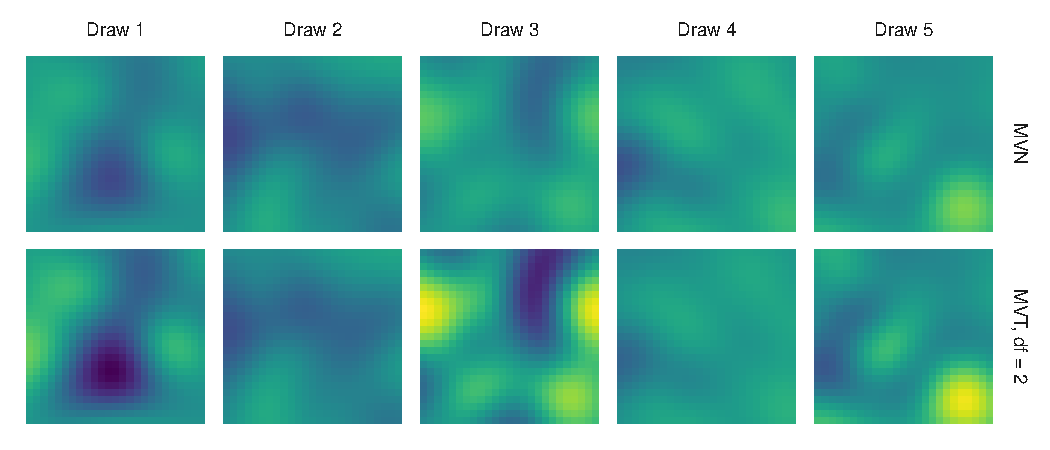
\includegraphics[width=0.9\textwidth]{../figs/nu-rf-illustration.pdf}
\caption{An illustration of five draws from a MVN random field (top row)
vs.\ five draws from a MVT random field with heavy tails            
(degrees of freedom, $\nu$, of 2; bottom row). Random seeds are held constant
between the rows
to illustrate the effect. Draws represent slices of time with independent spatial 
processes at each time slice. Note the considerably more extreme values in 
the third draw for the MVT spatial process.}
\label{fig:didactic}
\end{center}
\end{figure}

\clearpage

\begin{figure}[htb]
\begin{center}
  \includegraphics[width=0.65\textwidth]{../figs/sim-recapture-small.pdf}
\caption{Results from simulation testing the ability to recapture the degree 
of spatial heavy tailedness with varying number of time steps and varying 
true values of the degrees of freedom parameter, $\nu$. The number of time steps 
had the strongest effect on the ability to recapture $\nu$. Other elements to
the simulation testing are shown in Figure SXX. Dots show the 
median estimates from individual simulation runs and the polygons 
show the density. The color scale approximately indicates how heavy tailed 
the true distribution is: yellow (effectively normal), red (very heavy tailed).
}
\label{fig:didactic}
\end{center}
\end{figure}

\clearpage

\bibliography{spatial-extremes}

\end{spacing}
\end{document}

